\documentclass{article}
\usepackage[margin=1in]{geometry}
\usepackage{graphicx}
\usepackage{amsmath}
\usepackage{amssymb}
\usepackage{booktabs}
\usepackage{float}

\title{CSCI 567: Homework 2}
\author{anselzen@usc.edu (6163567905) and punyanay@usc.edu (8837304797)}
\date{September 27, 2026}

\begin{document}

\maketitle

\section*{Problem 1}

\subsection*{1.2}

\textbf{(b)}

\begin{center}
\begin{tabular}{lc}
\toprule
Quantity & Value \\
\midrule
Final training loss & 0.0755 \\
Training error rate & 0.0205 \\
Validation error rate & 0.0619 \\
$\|\mathbf{w}\|_2$ (bias excluded) & 11.223 \\
\bottomrule
\end{tabular}
\end{center}

\noindent
\textbf{(c)} It would be cheating because the min and max would then be computed using the
validation and test points too, so the model basically gets a peek at data it's supposed to
have never seen. That makes the validation and test error look better than they would on
actually unseen data.

\subsection*{1.3}

\textbf{(a)} Final training loss $= 1753.2952$, validation error rate $= 0.0973$.

\begin{figure}[H]
    \centering
    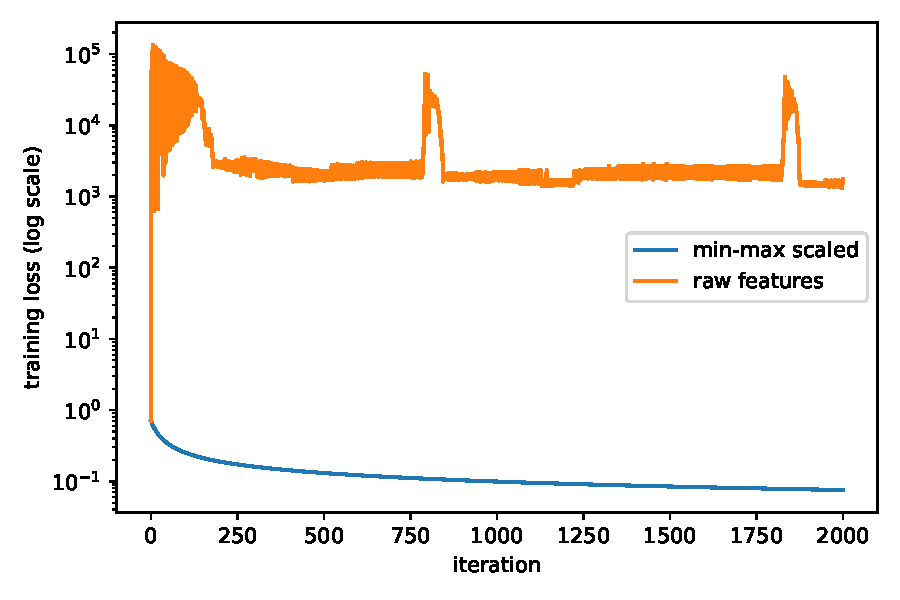
\includegraphics[width=0.7\textwidth]{logistic_loss_curves.pdf}
\end{figure}

\noindent
\textbf{(b)} Since some features are about $2000\times$ bigger than others, the loss gets super
steep in the directions of the big features' weights and almost flat in the others. So
$\eta = 0.5$ is way too big of a step for the steep directions: every step overshoots the minimum
and GD just bounces around (the loss shoots up to about $10^5$ and never settles) instead of going down.

\section*{Problem 2}

\subsection*{2.1}

\begin{center}
\begin{tabular}{cccccc}
\toprule
$\lambda$ & Objective & Loss & Train err & Val err & $\|\mathbf{w}\|_2$ \\
\midrule
0      & 0.0755 & 0.0755 & 0.0205 & 0.0619 & 11.223 \\
0.0001 & 0.0833 & 0.0775 & 0.0205 & 0.0531 & 10.818 \\
0.001  & 0.1300 & 0.0950 & 0.0293 & 0.0442 & 8.373 \\
0.003  & 0.1827 & 0.1252 & 0.0323 & 0.0442 & 6.195 \\
0.01   & 0.2683 & 0.1856 & 0.0469 & 0.0442 & 4.066 \\
0.03   & 0.3694 & 0.2697 & 0.0616 & 0.0619 & 2.578 \\
0.1    & 0.4907 & 0.3944 & 0.1056 & 0.1062 & 1.388 \\
1      & 0.6370 & 0.6082 & 0.3842 & 0.3186 & 0.240 \\
\bottomrule
\end{tabular}
\end{center}

\begin{figure}[H]
    \centering
    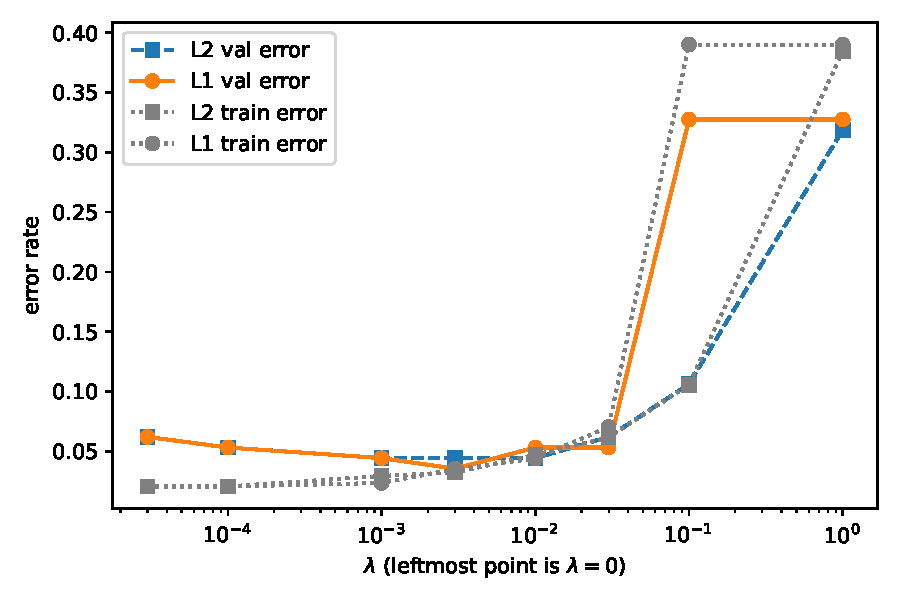
\includegraphics[width=0.7\textwidth]{reg_errors.pdf}
\end{figure}

\subsection*{2.2}

\textbf{(a)}
\[
\nabla \hat R_\lambda(\mathbf{w}) = \frac{1}{n}X^\top\big(\sigma(X\mathbf{w}) - \mathbf{y}\big) + \lambda\,\tilde{\mathbf{w}},
\qquad \tilde{\mathbf{w}} = (w_1, \ldots, w_{30}, 0).
\]
So it's the same gradient as Lecture 02, plus $\lambda w_j$ for every weight except the bias,
which gets $0$ since it isn't penalized.

\medskip
\noindent
\textbf{(b)} We pick $\lambda = 10^{-3}$, since it's the smallest $\lambda$ that gets the lowest
validation error ($0.0442$, tied with $3\cdot10^{-3}$ and $10^{-2}$).
When $\lambda$ is small, the weights are big and the model fits the training data too closely
(low bias, high variance: about $2\%$ training error vs.\ $6\%$ validation error), so adding a bit
of regularization brings the validation error down. But when $\lambda$ gets too big, the weights
get so small that the model can't even fit the training data anymore (high bias), so both errors
go up, which is why the validation curve goes down and then back up.

\section*{Problem 3}

\subsection*{3.1}

\begin{center}
\begin{tabular}{cccccc}
\toprule
$\lambda$ & Loss & Train err & Val err & $\|\mathbf{w}\|_2$ & \# nonzero \\
\midrule
0      & 0.0755 & 0.0205 & 0.0619 & 11.223 & 30 \\
0.0001 & 0.0765 & 0.0205 & 0.0531 & 10.999 & 30 \\
0.001  & 0.0872 & 0.0235 & 0.0442 & 9.468  & 26 \\
0.003  & 0.1090 & 0.0352 & 0.0354 & 8.299  & 14 \\
0.01   & 0.1687 & 0.0440 & 0.0531 & 6.789  & 7 \\
0.03   & 0.2967 & 0.0704 & 0.0531 & 5.189  & 3 \\
0.1    & 0.6688 & 0.3900 & 0.3274 & 0.000  & 0 \\
1      & 0.6688 & 0.3900 & 0.3274 & 0.000  & 0 \\
\bottomrule
\end{tabular}
\end{center}

\begin{figure}[H]
    \centering
    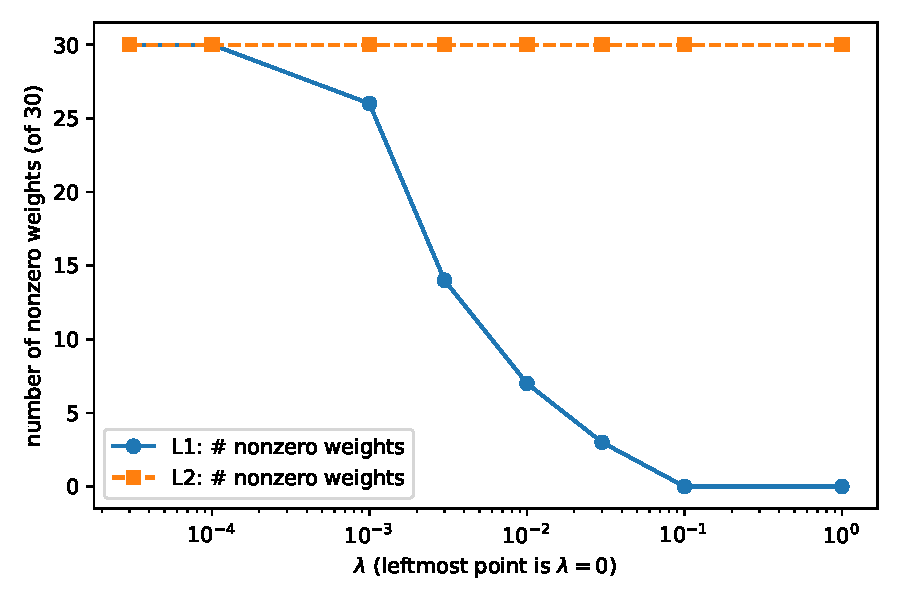
\includegraphics[width=0.7\textwidth]{sparsity.pdf}
\end{figure}

\subsection*{3.2}

\textbf{(a)} At $\lambda = 10^{-2}$, ridge sets $0$ of the 30 weights to exactly zero, but Lasso
sets $23$ of them to zero. This is because ridge's update multiplies each weight by
$(1-\eta\lambda)$, which makes it smaller but never exactly $0$, while Lasso's soft-threshold
subtracts $\eta\lambda$ and just snaps the weight to $0$ once $|v_j| \le \eta\lambda$.

\medskip
\noindent
\textbf{(b)} $\lambda = 10^{-2}$: mean concavity, mean concave points, worst radius, worst texture,
worst perimeter, worst area, worst concave points. $\lambda = 3\cdot10^{-2}$: worst radius, worst
perimeter, worst concave points. These make sense, since all the weights are positive, meaning
bigger tumors with more irregular, bumpy edges make the model more likely to say malignant.

\medskip
\noindent
\textbf{(c)} The sparsest model within one percentage point of the best is $\ell_1$ with
$\lambda = 3\cdot10^{-3}$ (validation error $0.0354$, which is actually the best overall),
and it uses 14 of the 30 features.

\section*{Problem 4: Kernel Logistic Regression}

\subsection*{4.2 The learned weights are label-signed residuals}

\subsubsection*{(a)}
We are given the gradient of the objective function:
\begin{equation*}
\nabla J(\alpha) = K \left[ \frac{1}{n}(\sigma(K\alpha) - y) + \lambda \alpha \right]
\end{equation*}
Letting $p = \sigma(K\alpha)$ denote the vector of fitted probabilities, we set the gradient to zero to find the minimizer:
\begin{equation*}
K \left[ \frac{1}{n}(p - y) + \lambda \alpha \right] = \mathbf{0}
\end{equation*}
Since the kernel matrix $K$ is given as invertible, we can multiply both sides from the left by $K^{-1}$:
\begin{align*}
\frac{1}{n}(p - y) + \lambda \alpha &= \mathbf{0} \\
\lambda \alpha &= \frac{1}{n}(y - p) \\
\alpha &= \frac{y - p}{n\lambda}
\end{align*}
Looking at this component-wise for each training point $i$, we obtain the desired identity:
\begin{equation*}
\alpha_i = \frac{y_i - p_i}{n\lambda}
\end{equation*}

\subsubsection*{(b)}
Let $\tilde{y}_i \in \{-1, +1\}$ denote the alternate class label notation corresponding to $y_i \in \{0, 1\}$. Because $p_i = \sigma(f_i)$, the probability values are strictly bounded within the open interval $(0, 1)$. We analyze the two cases for $y_i$:
\begin{itemize}
    \item \textbf{Case 1: $y_i = 1$ ($\tilde{y}_i = +1$).} Substituting $y_i = 1$ gives $\alpha_i = \frac{1 - p_i}{n\lambda}$. Since $0 < p_i < 1$, the numerator satisfies $0 < 1 - p_i < 1$. Thus, $\alpha_i > 0$, meaning $\text{sign}(\alpha_i) = +1 = \tilde{y}_i$, and $0 < |\alpha_i| < \frac{1}{n\lambda}$.
    \item \textbf{Case 2: $y_i = 0$ ($\tilde{y}_i = -1$).} Substituting $y_i = 0$ gives $\alpha_i = \frac{0 - p_i}{n\lambda} = -\frac{p_i}{n\lambda}$. Since $0 < p_i < 1$, the numerator satisfies $0 < p_i < 1$. Thus, $\alpha_i < 0$, meaning $\text{sign}(\alpha_i) = -1 = \tilde{y}_i$, and $0 < |\alpha_i| < \frac{1}{n\lambda}$.
\end{itemize}
Combining both cases, we can express $\alpha_i$ as the product of its magnitude and sign: $\alpha_i = |\alpha_i|\tilde{y}_i$. Substituting this back into the model's score function yields:
\begin{equation*}
f(x) = \sum_{i=1}^n \alpha_i \kappa(x, x_i) = \sum_{i=1}^n |\alpha_i| \kappa(x, x_i) \tilde{y}_i
\end{equation*}

\subsubsection*{(c)}
In words:
\begin{itemize}
    \item \textbf{Large Weight:} Training points that are misclassified or sit very close to the decision boundary receive large weights ($|\alpha_i| \approx \frac{1}{n\lambda}$). This occurs because their fitted probability $p_i$ is far from the true label $y_i$, creating a large residual.
    \item \textbf{Small Weight:} Training points that are correctly and securely classified deep within their true class regions receive small weights ($|\alpha_i| \approx 0$). For these points, $p_i \approx y_i$, making the residual negligible.
    \item \textbf{Role of $\lambda$:} The parameter $\lambda$ controls the regularizing constraint. A larger $\lambda$ shrinks the maximum possible weight capacity ($\frac{1}{n\lambda}$), forcing the model to look globally at all points to smooth out the boundary and prevent overfitting.
\end{itemize}

\subsection*{4.3 The two limits}

\subsubsection*{(a)}
As $\gamma \to \infty$, the RBF kernel function $\kappa(x, x_i) = \exp(-\gamma \|x - x_i\|^2)$ decays to 0 extremely fast for any non-identical points ($x \neq x_i$). For any evaluation point $x$, the kernel evaluation of its geometrically nearest training neighbor $x_j$ exponentially dominates all other components in the summation since the ratio $\kappa(x, x_i) / \kappa(x, x_j) \to 0$ for all $i \neq j$. Thus, the sign of both prediction scores becomes entirely determined by the nearest point, matching a 1-Nearest Neighbor (1-NN) classifier.

From the starter script execution, at $\gamma = 1000$, the weighted vote agrees with 1-NN on \textbf{1.000} of the validation points, while kernel logistic regression agrees on \textbf{0.914} of the validation points. 

Kernel logistic regression's agreement fraction is lower because it uses optimized, uneven weights $\alpha_i$ learned from training. At a large but finite value like $\gamma = 1000$, a nearby point with a massive learned magnitude $|\alpha_i|$ can still override a slightly closer point that has a near-zero weight. The unlearned weighted vote treats all labels with equal baseline magnitude, meaning the closest point dominates purely based on distance.

\subsubsection*{(b)}
As $\gamma \to 0$, the kernel values flatten to $\kappa(x, x_i) \to 1$ everywhere regardless of coordinate geometry. The decision functions become constant spatial baselines: the weighted vote predicts the global majority label based on the sign of the sum of $\tilde{y}_i$, and kernel logistic regression predicts the global weighted majority based on the sign of the sum of $\alpha_i$. 

In neighborhood heuristics, the neighborhood parameter $k$ (where $\gamma \propto 1 / k$) in $k$-NN, controls the inverse role of $\gamma$.

\subsection*{4.4 Balanced Rings}

\begin{center}
\begin{tabular}{ccc}
\toprule
$\gamma$ & Weighted Vote Error & Kernel Logistic Error \\
\midrule
0.1   & 0.496 & 0.058 \\
0.3   & 0.310 & 0.048 \\
1.0   & 0.080 & 0.044 \\
3.0   & 0.056 & 0.048 \\
10.0  & 0.046 & 0.056 \\
100.0 & 0.058 & 0.060 \\
1000.0& 0.060 & 0.122 \\
\bottomrule
\end{tabular}
\end{center}

\begin{figure}[H]
    \centering
    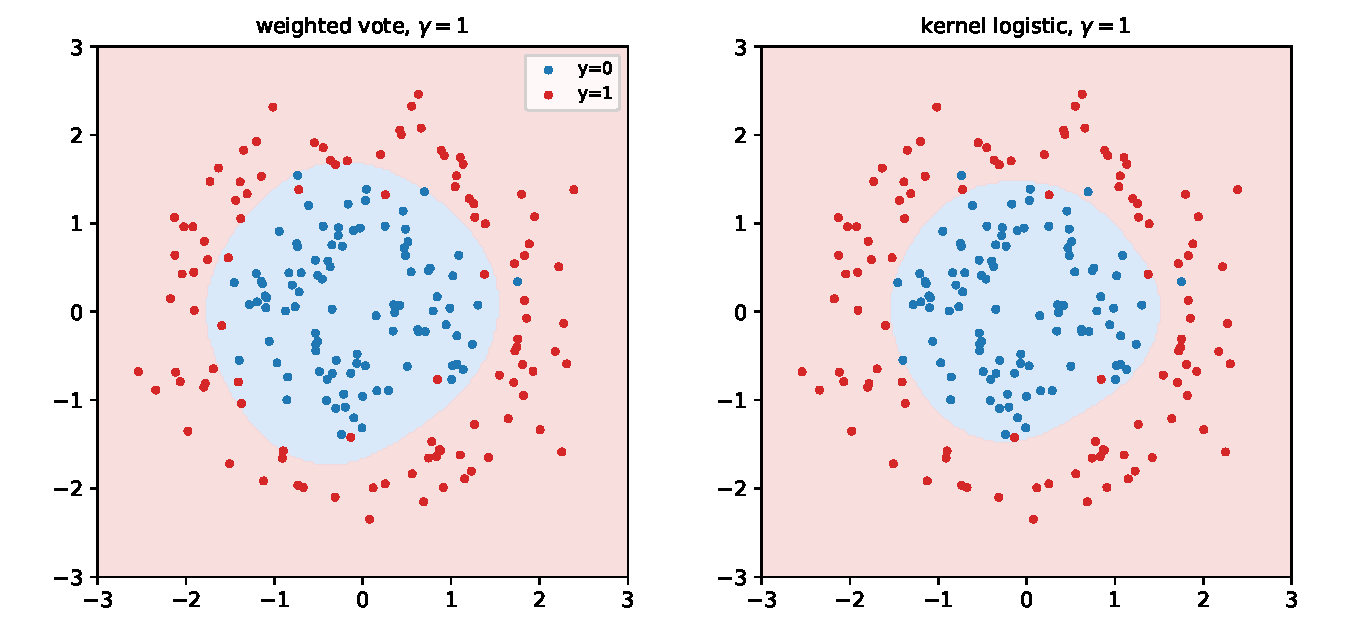
\includegraphics[width=0.7\textwidth]{balanced_boundaries.pdf}
\end{figure}

\subsubsection*{(a)}
Based on the validation sweep, the unlearned weighted vote is only effective over a narrow, localized range of higher values ($\gamma = 3$ to $\gamma = 100$), reaching its best error of 0.046 at $\gamma = 10$. In contrast, kernel logistic regression is highly robust across an intermediate-to-large spectrum ($\gamma = 0.1$ to $\gamma = 100$), maintaining low validation errors between 0.044 and 0.060. Both methods perform poorly at the extreme limits ($\gamma = 0.1$ for the vote, and $\gamma = 1000$ for kernel logistic regression).

\subsubsection*{(b)}
The best validation error rates for each method compare as follows:
\begin{itemize}
    \item \textbf{Kernel Logistic Regression:} 0.044 (achieved at $\gamma = 1$)
    \item \textbf{$k$-NN:} 0.056 (achieved at $k = 5$)
    \item \textbf{Weighted Vote:} 0.046 (achieved at $\gamma = 10$)
\end{itemize}
Kernel logistic regression achieves the lowest overall error rate among all three approaches.

\subsection*{4.5 Uneven density}

\subsubsection*{(a)}
\begin{center}
\begin{tabular}{ccccc}
\toprule
$\gamma$ & Vote All & Vote Left & KLR All & KLR Left \\
\midrule
0.3  & 0.138 & 0.155 & 0.072 & 0.099 \\
1.0  & 0.104 & 0.143 & 0.078 & 0.106 \\
3.0  & 0.086 & 0.124 & 0.070 & 0.093 \\
10.0 & 0.072 & 0.093 & 0.072 & 0.093 \\
\bottomrule
\end{tabular}
\end{center}

\begin{figure}[H]
    \centering
    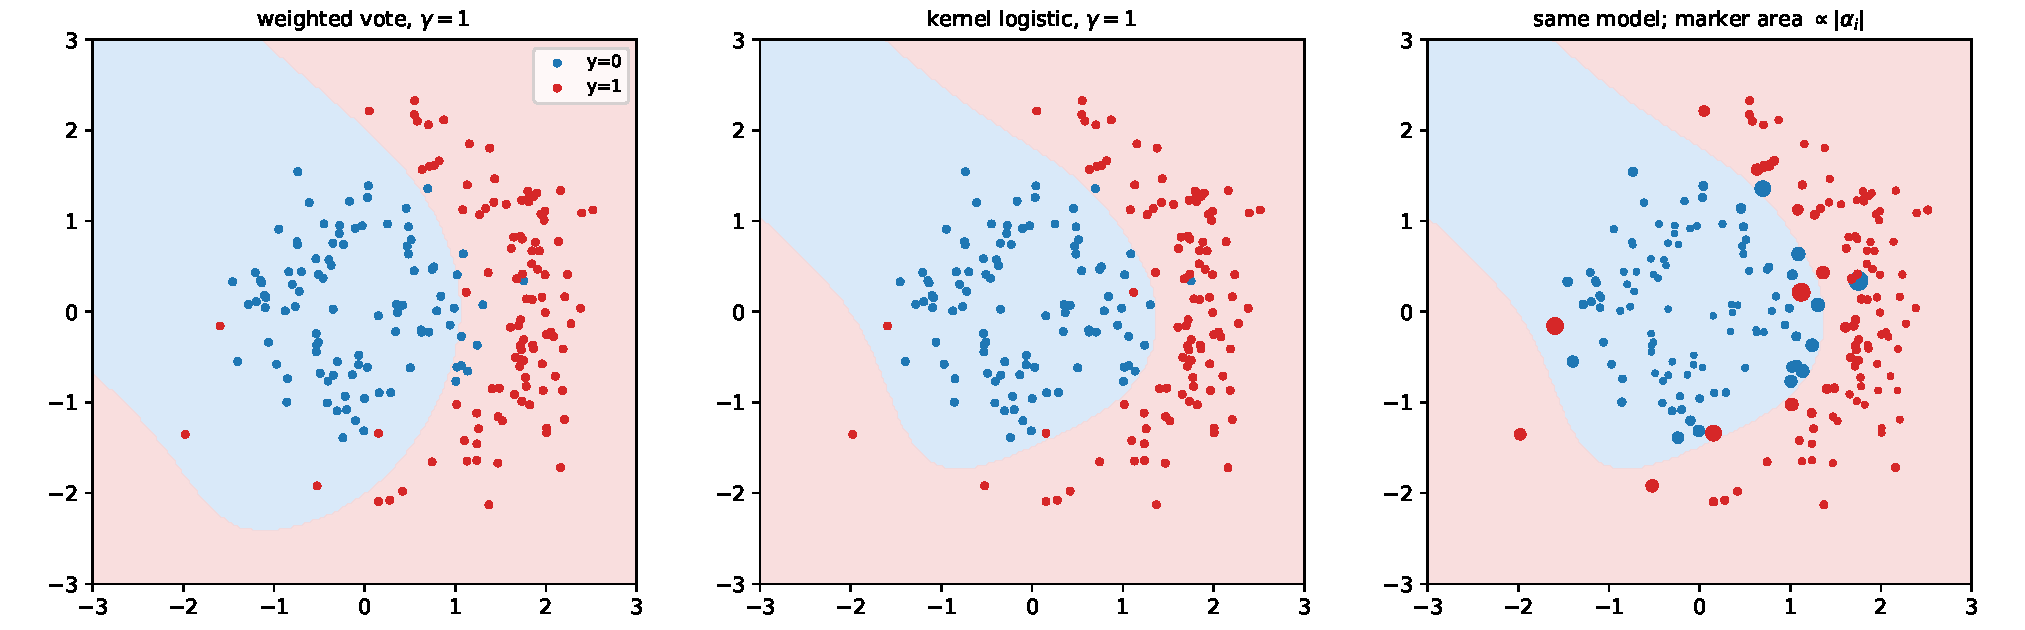
\includegraphics[width=0.9\textwidth]{uneven_boundaries.pdf}
\end{figure}

The decision boundary of the heuristic weighted vote breaks down drastically on the left side of the plane (yielding a high validation error of $0.143$ at $\gamma = 1.0$). 
On the left side, Class 1 points are highly sparse (forming only $5\%$ of the local dataset), while Class 0 remains uniformly dense. Because the unlearned vote assigns a fixed weight magnitude of $1$ to every single point, the massive regional volume of Class 0 neighbors completely dominates the score sum $s(x)$. 
This causes the summation to remain negative, flattening the decision boundary and misclassifying the sparse outer ring.

\subsubsection*{(b)}
The quantitative results from our empirical verification are as follows:
\begin{itemize}
    \item \textbf{Identity Check:} The predictions generated from the residual-defined weights $\beta$ agree with the trained coefficients $\alpha$ on \textbf{0.994} of the validation points. The maximum weight magnitude is $\max |\beta| = 4.654$, which is strictly bounded below the theoretical cap of $1 / (n\lambda) = 5.0$. The condition $\operatorname{sign}(\beta) = 2y - 1$ holds perfectly across \textbf{1.000} of the points.
    \item \textbf{Mean Weight Magnitudes ($|\beta|$):}
    \begin{itemize}
        \item Class 1: Left half (sparse) = \textbf{2.148}, Right half (dense) = \textbf{0.366}
        \item Class 0: Left half (dense) = \textbf{0.222}, Right half (sparse) = \textbf{0.662}
    \end{itemize}
\end{itemize}

This happens because the weights follow the formula $\alpha_i = (y_i - p_i) / (n\lambda)$, meaning a point's weight depends entirely on its prediction error. On the left side, Class 1 points are rare, so the model struggles to predict them ($p_i \approx 0$). This leaves a huge residual ($1 - p_i \approx 1$), forcing their average weight magnitude up to a massive $2.148$. On the right side, Class 1 points are surrounded by matching neighbors, making them easy to predict correctly ($p_i \approx 1$). This shrinks the error, keeping their average weight tiny ($0.366$).

This adaptive weight pattern is how kernel logistic regression fixes the boundary. By automatically blowing up the weights of the sparse points on the left, a few Class 1 points can hold their ground against a whole crowd of dense Class 0 neighbors. Simple heuristics like $k$-NN or a regular weighted vote fail here because they treat every point the same. They cannot adjust their sensitivity based on local data density, causing them to get overwhelmed.

\end{document}
